\documentclass[12pt]{article}
\usepackage[all, stdclass]{lix}
\usepackage{graphicx}
\usepackage{svg}
\usepackage{circuitikz}
\svgsetup{
  inkscapepath=assets/,  % Path to the directory containing your SVG files
  svgpath=assets/        % Path to the directory containing your SVG files
}
\usepackage{float}
\usepackage{hyperref}
\usepackage{times}
\usepackage{amsmath}
\usepackage{pgfplots}
\usepackage{pdfpages}

%----------EDIT COVER INFO HERE -----------------%

\def \LOGOPATH {assets/birzeit-logo.png}
\def \DEPARTEMENT {Department of Electrical \& Computer Engineering}
\def \COURSENUM {ENEE2103}
\def \COURSENAME {Circuits and Electronics Laboratory}
\def \REPORTTITLE {Filed-Effect Transistor (FET)}
\def \STUDENTNAME {Mohammad Abu-Shelbaia}
\def \STUDENTID {1200198}
\def \INSTRUCTOR {Dr. Mahran Quraan}
\def \ASSISTANT {Eng. Rafah Rahhal}
\def \PARTNERAN {Nidal Zabade}
\def \PARTNERBN {Mahmoud Shihab}
\def \PARTNERAID {1200153}
\def \PARTNERBID {1182143}
\def \REPORTNUM {8}

\begin{document}
\pagenumbering{Roman}

\begin{titlepage}
    \vfill
    \begin{center}
        \includegraphics[width=0.7\textwidth]{\LOGOPATH} \\
        \hfill \\
        \Large{\DEPARTEMENT} \\
        \Large{\COURSENUM\;-\;\COURSENAME} \\
        \vfill
        \textbf{\LARGE{Experiment \#\REPORTNUM}} \\
        \textbf{\LARGE{\REPORTTITLE}}
    \end{center}
    \vfill
    \begin{flushleft}
        \Large{\textbf{Prepared by:}\\ \STUDENTNAME\quad\STUDENTID} \\
        \Large{\textbf{Partners:}\\ 
        \begin{tabular}{@{}l@{\quad}l}
            \PARTNERAN & \PARTNERAID \\
            \PARTNERBN & \PARTNERBID \\
        \end{tabular}} \\
        \Large{\textbf{Instructor:} \INSTRUCTOR} \\
        \Large{\textbf{Assistant:} \ASSISTANT} \\
        \Large{\textbf{Section:} 4}\\
        \LARGE{\textbf{ }}\\
        \LARGE{\textbf{ }}\\
        \LARGE{\textbf{ }}\\
        \Large{\textbf{Date:} \today}\\
    \end{flushleft}
    \vfill
\end{titlepage}
{
\centering
\section*{Abstract}
This experiment demonstrates the difference between the Bipolar Junction Transistor (BJT) and the Junction Field-Effect Transistor (FET),  the characteristics of the JFET, and how to use it as an amplifier. It also shows how to use the JFET as a common drain amplifier (SOURCE FOLLOWER).
}
\clearpage

%--------------- TABLES --------------------------------%
\tableofcontents
\clearpage
\setlength{\parskip}{\baselineskip}%
\listoffigures
\clearpage
\listoftables
\clearpage
\pagenumbering{arabic}
%-------------- CONTENT ---------------------%
\h{Theory}
\hh{Junction Filed-Effect Transistor (JFET)}

The field-effect transistor is eithar a Metal Oxide Semeiconductor Filed-Effect Transitor (MOSFET) or a Junction Field-Effect Transistor (JFET).

The JFET's are split into two, either n-channel or p-channel. The n-channel JFET has a n-type semiconductor between two p-type semiconductors, while the p-channel JFET has a p-type semiconductor between two n-type semiconductors.
\begin{figure}[H]
    \centering
    \begin{circuitikz}[american]
        \draw (0,0) node[njfet] (n1) {N-Channel};
        \draw (n1.G) to[short,-o] ++(-0.3,0) node[left] {G};
        \draw (n1.D) to[short,-o] ++(0,0.3) node[above] {D};
        \draw (n1.S) to[short,-o] ++(0,-0.3) node[below] {S};
        
        \draw (4,0) node[pjfet] (n2) {P-Channel};
        \draw (n2.G) to[short,-o] ++(-0.3,0) node[left] {G};
        \draw (n2.D) to[short,-o] ++(0,-0.3) node[below] {D};
        \draw (n2.S) to[short,-o] ++(0,+0.3) node[above] {S};
        
    \end{circuitikz}
    \caption{JFETs (n-channel and p-channel)}
\end{figure}
The main different between JFET's and BJT is that the JFET is a voltage controlled device, while the BJT is a current controlled device. The JFET is controlled by the voltage between the gate and the source, while the BJT is controlled by the current between the base and the emitter.

JFET's has higher input impedance than BJT's, however they have lower gain. JFET's are also more temperature stable than BJT's which makes them useful in integrated circuits.
The main characteristics of the JFET is the pinch-off voltage $V_{p}$, the drain current $I_{D}$, and the transconductance $g_{m}$. 

The pinch-off voltage is the voltage between the gate and the source at which the drain current is zero. The drain current is the current flowing from the drain to the source. The transconductance is the ratio between the change in the drain current and the change in the gate-source voltage.
\hh{Transconductance}
The transconductance is the ratio between the change in the drain current and the change in the gate-source voltage. The transconductance is given by:
\begin{equation}
    g_m = \frac{\Delta I_D}{\Delta V_{GS}}
\end{equation}
\hh{Common Source Amplifier}
in this configuration the circuit acts as an amplifier, the voltage gain is higher in comparsion with the common drain amplifier, and the output voltage is out of phase with the input voltage (180$^{\circ}$). The input impedance is high, while the output impedance is low. And the gain is given by:
\begin{equation}
    A_v = - \frac{g_m\times R_D}{1 + g_m\times R_D}
\end{equation}
Where $g_m$ is the transconductance and $R_D$ is the drain resistor. 
\hh{Common Drain Amplifier (Source Follower)}
\begin{figure}[H]
  \centering
  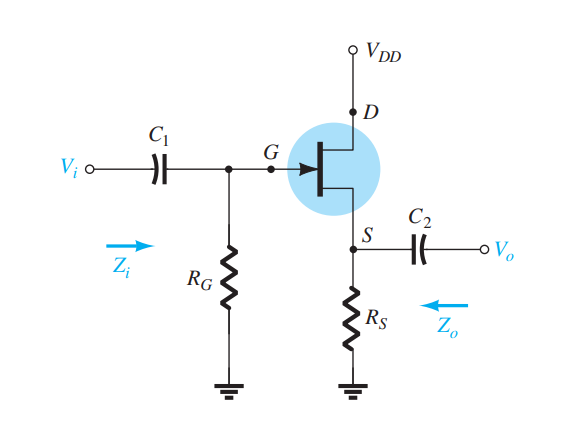
\includegraphics[width=0.5\textwidth]{assets/main/2023-08-26-12-11-17.png}
  \caption{Common Drain Amplifier}
  \cite{book}
\end{figure}
in this configuration the circuit acts as a voltage follower, the output is connected to the source while the input is connected to the gate. The voltage gain is less than 1, and the output voltage is in phase with the input voltage. The input impedance is high, while the output impedance is low. And the gain is given by:
\begin{equation}
    A_v = \frac{g_m\times R_S}{1 + g_m\times R_S}
\end{equation}
Where $g_m$ is the transconductance and $R_S$ is the source resistor.
\clearpage
\h{Procedure and Data Analysis}
\hh{Characteristics of N-Channel JFET}
\begin{figure}[H]
    \centering
    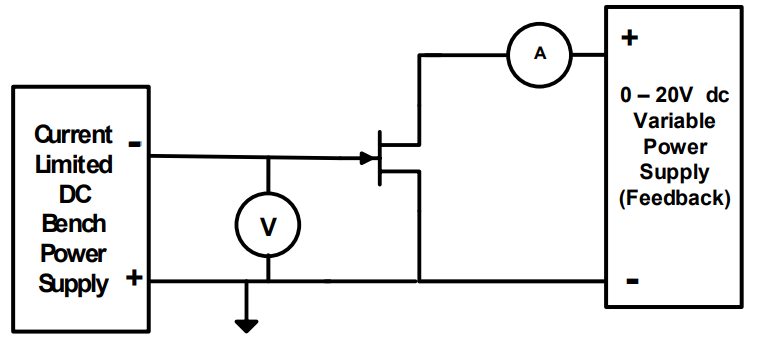
\includegraphics[width=0.7\textwidth]{assets//main/2023-08-25-16-10-51.png}
    \caption{N-Channel JFET Characteristics Circuit}
\end{figure}
The circuit above was connected, and the following values were measured by reading different values for $I_D$ at values for $V_{DS}$ ranging from 0 to 15V for $V_{GS}$ ranging from 0 to -2.5V. The results are shown in Table \ref{tab:my-table} and Figure \ref{fig:my-figure}.
\begin{table}[H] % Table 1
    \centering
    \resizebox{0.7\textwidth}{!}{%
    \begin{tabular}{|c|ccccccc|}
    \hline
     &
      \multicolumn{7}{c|}{$I_D$(mA) for $V_{DS}$} \\ \hline
    $V_{GS}$ &
      \multicolumn{1}{c|}{0} &
      \multicolumn{1}{c|}{0.5} &
      \multicolumn{1}{c|}{1} &
      \multicolumn{1}{c|}{2} &
      \multicolumn{1}{c|}{5} &
      \multicolumn{1}{c|}{10} &
      15 \\ \hline
    0 &
      \multicolumn{1}{c|}{0.0339} &
      \multicolumn{1}{c|}{1.2} &
      \multicolumn{1}{c|}{2.8} &
      \multicolumn{1}{c|}{4.7} &
      \multicolumn{1}{c|}{5.8} &
      \multicolumn{1}{c|}{6} &
      6 \\ \hline
    -0.5 &
      \multicolumn{1}{c|}{0.0347} &
      \multicolumn{1}{c|}{1.1} &
      \multicolumn{1}{c|}{2.4} &
      \multicolumn{1}{c|}{3.6} &
      \multicolumn{1}{c|}{4.5} &
      \multicolumn{1}{c|}{4.7} &
      4.7 \\ \hline
    -1 &
      \multicolumn{1}{c|}{0.0333} &
      \multicolumn{1}{c|}{0.91} &
      \multicolumn{1}{c|}{1.35} &
      \multicolumn{1}{c|}{2.45} &
      \multicolumn{1}{c|}{3.29} &
      \multicolumn{1}{c|}{3.75} &
      3.63 \\ \hline
    -1.5 &
      \multicolumn{1}{c|}{0.0331} &
      \multicolumn{1}{c|}{0.7} &
      \multicolumn{1}{c|}{1.22} &
      \multicolumn{1}{c|}{1.57} &
      \multicolumn{1}{c|}{1.76} &
      \multicolumn{1}{c|}{1.82} &
      1.85 \\ \hline
    -2 &
      \multicolumn{1}{c|}{0.0285} &
      \multicolumn{1}{c|}{0.52} &
      \multicolumn{1}{c|}{0.75} &
      \multicolumn{1}{c|}{0.89} &
      \multicolumn{1}{c|}{0.97} &
      \multicolumn{1}{c|}{1.01} &
      1.03 \\ \hline
    -2.5 &
      \multicolumn{1}{c|}{0.0225} &
      \multicolumn{1}{c|}{0.24} &
      \multicolumn{1}{c|}{0.25} &
      \multicolumn{1}{c|}{0.31} &
      \multicolumn{1}{c|}{0.34} &
      \multicolumn{1}{c|}{0.36} &
      0.37 \\ \hline
    \end{tabular}%
    }
    \caption{N-Channel JFET Characteristics}
    \label{tab:my-table}
\end{table}
\begin{figure}[H] % Figure 1
    \centering
    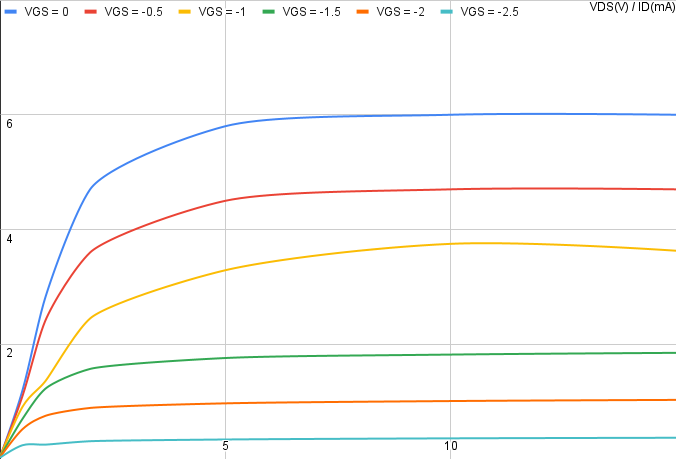
\includegraphics[width=0.5\textwidth]{assets/chart (17).png}
    \caption{N-Channel JFET Characteristics Curves}
    \label{fig:my-figure}
\end{figure}
According to the results in Table \ref{tab:my-table} and Figure \ref{fig:my-figure}, the pinch-off voltage is $|V_p|\approx 10V$, since at $V_{GS} = 0V$ the drain current is constant after $V_{DS} = 10V$. Furthermore at the pinch-off voltage and $V_{GS} = -1.0V$ the $I_G$ is very small since at the pinch-off voltage the drain current is taking using most of the current. 

The transconductance is:
\begin{equation}
    g_m = \frac{\Delta I_D}{\Delta V_{GS}} = \frac{I_{D2} - I_{D1}}{V_{GS2} - V_{GS1}} = \frac{3.75 - 1.01}{-1 - (-2)} = 2.74 \frac{mA}{V}
    \label{eq:gm}
\end{equation}
\hh{JFET as an Amplifier}
\begin{figure}[H]
    \centering
    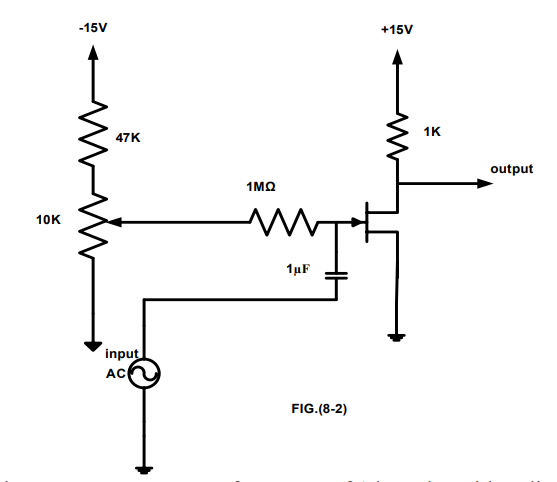
\includegraphics[width=0.5\textwidth]{assets/main/2023-08-25-18-20-27.png}
    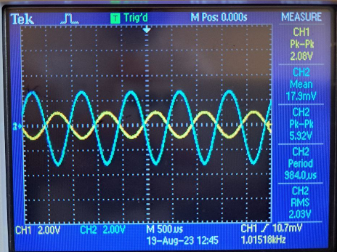
\includegraphics[width=0.49\textwidth]{assets//main/2023-08-25-18-29-02.png}
    \caption{JFET Amplifier Circuit}
\end{figure}
The circuit above was connected to a function generator and an oscilloscope. The function generator was set to produce a 1kHz sine wave with 2V peak-to-peak. The potentomiter was set to give a value of $V_{DS} = 10V$, The oscilloscope was connected to the input and output of the circuit and the following results were obtained.
The gain is:
\begin{equation}
    A_v = \frac{V_{out}}{V_{in}} = \frac{5.92}{2.08} = 2.85
\end{equation}
The input impedance is:
\begin{equation}
    Z_{in} = \frac{V_{in}}{I_{in}} = \frac{0.707}{38.4 \mu} =  18.4 k\Omega
\end{equation}
We noticed that the ampilfer gain is low in comparsion with the bjt amplifier, this is because the JFET has a lower transconductance than the BJT. The input impedance is higher than the BJT amplifier, this is because the JFET has a higher input impedance than the BJT.
\hh{Common Drain Amplifier}
\begin{figure}[H]
    \centering
    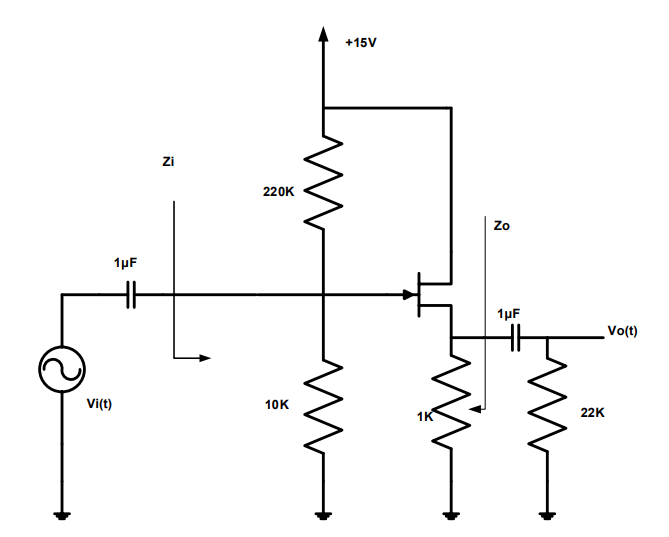
\includegraphics[width=0.49\textwidth]{assets/main/2023-08-25-18-33-54.png}
    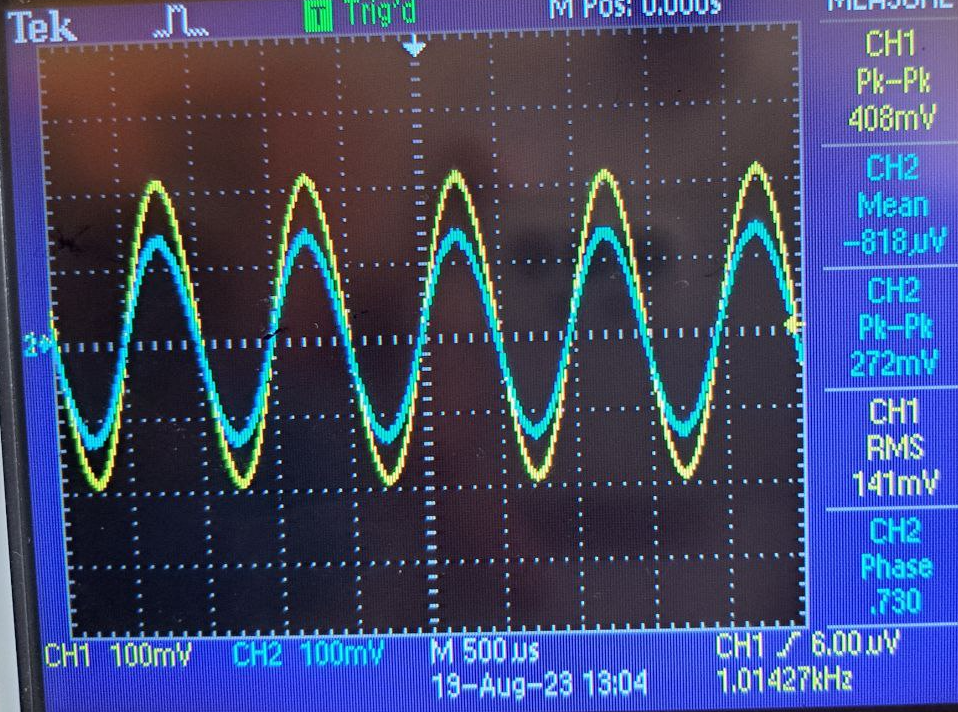
\includegraphics[width=0.49\textwidth]{assets//main/2023-08-25-18-42-04.png}
    \caption{Common Drain Amplifier}
\end{figure}
The circuit above was initialy connected without the AC source, and the following values were measured $V_G$ = 0.645 and $V_S$ = 2V. The AC source was connected and the function generator was set to produce a 1kHz sine wave with 2V peak-to-peak. The oscilloscope was connected to the input and output of the circuit and the following results were obtained.
The gain is:
\begin{equation}
    A_v = \frac{V_{out}}{V_{in}} = \frac{272mV}{408mV} = 0.667
\end{equation}
The phase shift is 0.730$^{\circ} \approx 0$ and the input and output impedances:
\begin{equation}
    Z_{in} = \frac{V_{in}}{I_{in}} = \frac{140m}{39 \mu} = 3.58 k\Omega
\end{equation}
  
\begin{equation}
    Z_{out} = \frac{V_{out}}{I_{out}} = \frac{39.43}{37.77 \mu} = 1.04k\Omega
\end{equation}

The theoritical gain is:
\begin{equation}
    A_v = \frac{g_m\times R_S}{1 + g_m\times R_S} = \frac{0.00274\times 1k}{1 + 0.00274\times 1k} =  0.733
\end{equation}
the theoritical gain is close to the measured gain and it doesn't excced 1 because the common drain amplifier is a voltage follower.
\clearpage
\h{Conclusion}
In conclusion, we learned the characteristics of the JFET, and how to use it as an amplifier. We also learned how to use the JFET as a common drain amplifier (SOURCE FOLLOWER), Finally we learned the difference between the Bipolar Junction Transistor (BJT) and the Junction Field-Effect Transistor (JFET).
\clearpage
\bib{cites}
\clearpage
\h*{Appendix}
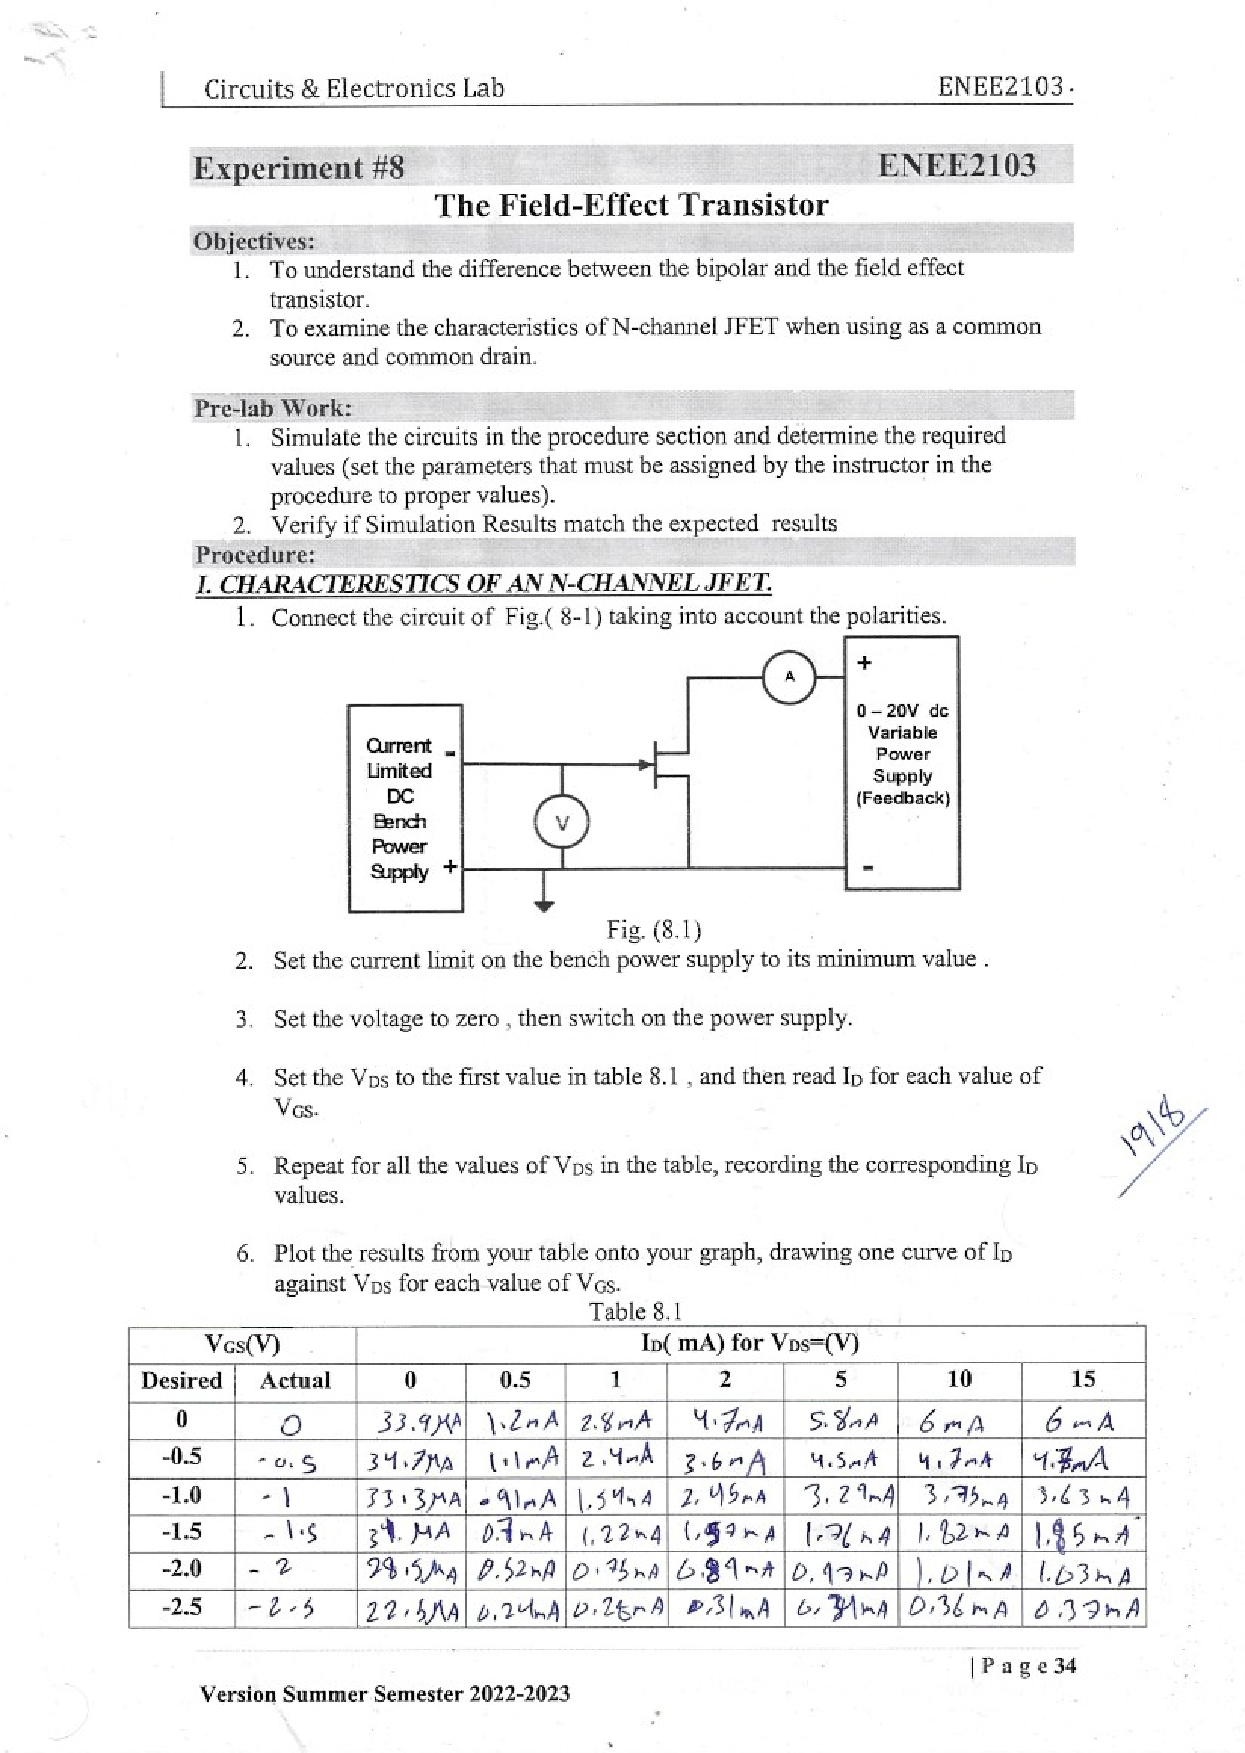
\includepdf[pages=-]{2023-08-25_015081.pdf}
\clearpage
\end{document}





